\documentclass[a4paper,10pt]{article}
\usepackage[dutch]{babel}
\usepackage[utf8]{inputenc}
\usepackage{helvet,graphicx,geometry,fancyhdr,parskip,tocloft,listings,icomma,hyperref,textcomp}
%
% kantlijnen
\geometry{left=2cm,right=2cm,top=3cm,bottom=2.5cm}
%
% schreefloos lettertype
\let\familydefault\sfdefault
%
% listings
\lstset{numbers=left,basicstyle=\ttfamily\small}
%
% header en footer
\pagestyle{fancy}
\renewcommand{\headrulewidth}{0pt}
\renewcommand{\footrulewidth}{.4pt}
\setlength{\headheight}{33pt}
\lhead{\hrulefill\\[-1mm]\MakeUppercase{\footnotesize practicumhandleiding tincps02-1\hfill{}Hogeschool Rotterdam/CMI}\hspace{1cm}\raisebox{-8mm}{\includegraphics[width=1cm]{HR_LOGO_rechtsonder_CMYK_rood1}}}
\rhead{}
\lfoot{\footnotesize\MakeUppercase\today}
\cfoot{}
\rfoot{\footnotesize\thepage}
%
% section headings
\let\mysection\thesection
\renewcommand\thesection{Les \mysection:}
\setlength{\cftsecnumwidth}{4em}
%
% code
\newcommand{\code}[1]{\texttt{#1}}
%
% titelpagina
\begin{document}
\begin{center}
\vspace*{4cm}
\MakeUppercase{\Large\bfseries Hogeschool Rotterdam / CMI}\\
\vspace{3cm}
\textbf{\fontsize{48}{60}\selectfont Practicumhandleiding Programmeren 2: Object-geori"enteerd Programmeren}\\
\vspace{2cm}
\MakeUppercase{\Large\bfseries tinpro02-2}\\
\end{center}
\vspace{4cm}
\begin{tabbing}
Cursusjaar: \=2018--2019\\
Auteurs:\>dr.\ W.\ M.\ Bergmann Tiest\\
\>ir.\ J.\ de Hooge
\end{tabbing}
\newpage
%
% inhoudsopgave
\tableofcontents
\newpage
%
% lessen
In deze cursus ga je stap voor stap de besturing van een voertuig maken dat zich door een wereld beweegt waarin zich obstakels bevinden, en dat een doellokatie in de wereld moet bereiken. Deze virtuele wereld wordt gegeven. Het is jouw opdracht om classes te maken die het voertuig en de besturing implementeren. Je voertuig krijgt via sensoren signalen binnen (afstand en richting) van alle obstakels in de wereld en van het doel. De bedoeling is om de obstakels te ontwijken en het doel te bereiken. Het voertuig moet beginnen op positie (0,0) met ori"entatie 0\textdegree{}. Positieve hoeken gaan tegen de klok in (voor de zeilers onder jullie: dit is omgekeerd aan een gewoon kompas).\\
\centerline{\includegraphics[width=12cm]{world}}
\section{Initializing}
Maak een java-programma \code{Program.java} dat de tekst ``Initializing self-driving vehicle\dots'' op de console print.
\section{Classes en Objecten}
Maak een class \code{MotorizedWheel} en een class \code{Vehicle} die twee van deze wielen heeft: \code{leftWheel} en \code{rightWheel}. Zorg dat deze wielen in de constructor van \code{Vehicle} ge"instantieerd worden. Maak eerst een klassediagram. Breid de \code{main()} method van class \code{Program} uit zodat er een instance van \code{Vehicle} gemaakt wordt.

\section{Public en private (inleveropgave, formatief)}

De class \code{Vehicle} moet de volgende public methods hebben:
\begin{lstlisting}
void addSignal(Signal s)
Position drive(double dt)
void bounceBack(Position p)
Position getPosition()
double getOrientation()
\end{lstlisting}
Tevens moet de class \code{Vehicle} een private method \code{void updateVehicle(double dt)} hebben. Maak \textit{stubs} aan voor deze methods. De classes \code{Signal} en \code{Position} zijn gegeven (zie \code{World.java}). Bedenk welke fields en methods je nog meer nodig hebt, en of deze public of private moeten zijn.

\subsection*{Inkapseling in Java}

Het is in Java o.a. mogelijk te kiezen welke functies en velden van een klasse wel en welke niet voor objecten van andere klassen toegankelijk zijn.
Ook bij de eindopdracht is deze keuze van belang en we oefenen er hier in deze les alvast mee.
Het komt er op neer dat je je afvraagt wat nu eigenlijk van buitenaf bezien de essentie van iets is.
Een essentiele ``activiteit'' van een wegvoertuig is bijvoorbeeld dat 't kan rijden.
Of er een verbrandingsmotor of een electromotor in zit is van minder belang, behalve voor oliemaatschappijen.

Functies (methods) en velden van objecten die van buitenaf toegankelijk zijn, worden aangeduid met het woord \emph{public}.
Functies en velden die alleen vanuit objecten van de betreffende klasse zelf bruikbaar zijn, worden aangeduid met het woord \emph{private}.
De woorden \emph{public} en \emph{private} worden access class labels genoemd.
Er zijn er nog meer, maar die komen in latere lesseries aan de orde.

Het is nodig, bij het ontwerpen van je programma in een vroeg stadium te bedenken welke functies en velden \emph{public} moeten zijn, en welke \emph{private},
vooral als je programma groeit of anderszins verandert.
Het onderstaande verhaal, dat niet over computerprogramma's maar horloges gaat, maakt dit duidelijk.

\subsection*{Demetrius en z'n vrouw}

\begin{framed}
Demetrius was een goudsmid die horloges maakte.
Die horloges waren beroemd over de hele wereld en hij had altijd genoeg werk.

Vaak als hij over een horloge gebogen zat, kwam z'n vrouw binnen en riep: KOFFIEEE!!
Hij schrok hier soms zo van, dat hij z'n werk uit z'n handen liet vallen,
waarna het betreffende horloge in honderden tandwieltjes, veertjes en lagertjes uitelkaar spatte.
Soms vloekte hij dan in het latijn, wat beschaafder klonk dan het was.

Op zekere dag had hij een goed idee:
Hij besloot z'n horloges op te bouwen uit een beperkt aantal modules, die op zich stabiele eenheden vormden.
Als z'n vrouw binnenkwam, kon het nu hoogstens nog gebeuren dat het horloge uiteenviel in een stuk of twintig modules.
Of de laatste module, waar hij net aan bezig was, viel uiteen in enkele tientallen tandwieltjes, maar daar viel mee te leven.

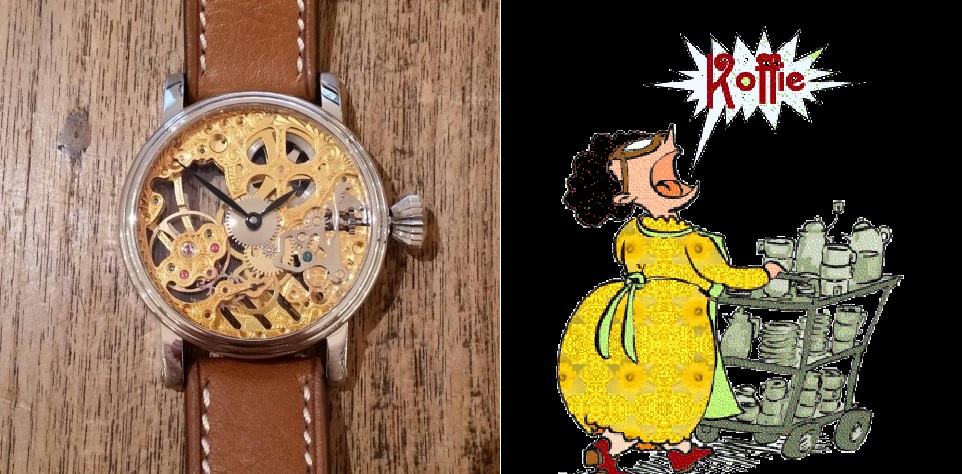
\includegraphics[width=12cm]{horloge_koffie}

Als hij er eens lekker zin in had, maakte hij een voorraadje van allerlei modules.
Wat hem echter dwars zat, is dat elke module eigenlijk maar in een soort horloge bruikbaar was.
Daarnaast ging het in elkaar schroeven van steeds maar weer de zelfde modules hem ook vervelen.

Hij schafte daarom een modulefabriekje aan, een soort robot avant la lettre.
Omdat hypes alleen ontstaan als je er wat nieuwe woorden voor verzint,
noemde hij z'n robotjes klassen, en de modules die er door werden gefabriceerd, objecten.

Wat bijzonder was aan die objecten, is dat ze zo waren ontworpen dat ze in meerder soorten horloges pasten.
Af en toe verbeterde hij z'n klassen, zodat ze efficientere objecten konden maken.
Hij zorgde er echter wel voor dat die nieuwe objecten in plaats van de oude konden worden gebruikt:
ze hadden de zelfde vorm en wijze van interactie met hun omgeving.
Omdat hij trots was op dit opnieuw briljante idee, verzon hij ook hier weer een woord voor: interface.

Hoewel zijn objecten dus een min of meer onveranderlijk interface hadden, was hij toch erg flexibel in z'n productie.
Immers kon hij de technologie binnen een object veranderen,
bijvoorbeeld van veermotor met onrustje naar kwartsgestabiliseerde synchroonmotor,
zonder dat dat enige consequenties had voor andere objecten in 't zelfde horloge,
zoals de wijzerplaat met wijzers of 't datummechanisme.

Zoals alle technici werd Demetrius er niet rijk van,
maar dat gaf niet, hij kon nu meer van z'n koffie genieten.
Zijn vondst, in de Romeinse tijd bekend als ``Divide et Impera'' (Verdeel en Heers),
heet tegenwoordig de ``Law of Demeter'' en vormt de grondslag voor Object Oriented Development.

\url{https://en.wikipedia.org/wiki/Law_of_Demeter}

Zoals je op bovenstaande webpage kunt lezen, is object orientatie geen panacee (middel tegen alle kwalen).
Het is echter wel succesvol genoeg om op ruime schaal ingang te vinden in de industrie.
Java is een typisch voorbeeld van een object georienteerde taal.
Door middel van gepast gebruik van \emph{public} en \emph{private} kun je duidelijk maken,
wat tot het interface van je objecten behoort, en wat interne details zijn, die eventueel kunnen wijzigen.
\end{framed}

\subsection*{Objectgeorienteerde chocoladerepen}

Demetrius' werkwijze kwam in de mode en allerlei programmeertalen, van PHP tot JavaScript, kregen opeens het stempel ``object georienteerd''.
Om het kaf van het koren te scheiden werd het noodzakelijk aan te geven waaraan een object georienteerde taal moet voldoen om die naam te verdienen.
Bij een object georienteerde taal zijn minimaal de volgende conceptuele elementen aanwezig:

\begin{itemize}

\item Inkapseling: Zoals besproken, het verbergen van ontwerpbeslissingen betreffende details en het onderbrengen van deze details in een gemeenschappelijk ``omhulsel''.
Een wijd verbreid misverstand is dat het hierbij gaat om het verbergen van data.
Het gaat echter om het verbergen van datgene wat veranderlijk is.
Soms is dat de data, soms de functies die op deze data werken.
Een goed interface (public part, zie code voorbeelden) is dun (laat niet te veel zien) en stabiel (onveranderlijk).
Immers alles wat je in het interface opneemt, kun je niet zo maar meer wijzigen.
En alles wat aan het interface moet veranderen, zorgt ervoor dat ook andere objecten moeten worden aangepast.
Inkapseling vormt de hoofdmoot van wat Demetrius deed met z'n horloges.

\item Overerving: Objecten die een speciaal geval vormen van andere objecten ondersteunen minimaal hetzelfde interface.
De belangrijkste regel hier is: Do not disinherit (onterf niet).
Een versterker met een extra aansluiting voor fibre optics is OK.
Een versterker zonder cinch aansluitingen is in veel gevallen niet inpasbaar in een bestaande audio-installatie.
Doen alsof je een vogel bent, maar niet kunnen vliegen is teleurstellend, hoewel struisvogels hier anders over denken.
Maar ja, die steken hun kop in 't zand...
Naast deze ``interface inheritance'' bestaat er ook implementation inheritance.
Hierbij draait het om ``hergebruik'' van broncode.
Aanvankelijk werd dit zelfs gebracht als HET argument om object georienteerd te werken.
Echter bleek al snel dat flaws net zo inheritable waren als features.
Inkapseling (HAS A) van bestaande code bleek in veel gevallen vruchtbaarder dan overerving ervan (IS A).
Voorbeeld: De aanname dat een computer een toetsenbord en een beeldscherm BEVAT, is correcter dan de aanname dat een computer zowel een toetsenbord als een beeldscherm IS.
En correcte aannamen over de fysische objecten leiden tot betere opbouw van software objecten die hiermee moeten communiceren.

\item Veelvormigheid: Een verzameling objecten (zoals een lijst) kan heel divers zijn, zolang ze maar allemaal hetzelfde interface ondersteunen.
Dit in tegenstelling tot bijvoorbeeld een relationele database, benaderbaar in SQL.
Alle regels (records) van een tabel hebben daar hetzelfde dataformaat.
De mogelijkheid verschillende soorten objecten in dezelfde datastructuur op te nemen, opent een wereld van flexibititeit.
Omdat diverse objecten via hun overeenkomstige interface toch op een overeenkomstige manier aangesproken kunnen worden,
neemt bij gebruik van veelvormigheid de grootte van de broncode sterk af.
Immers dezelfde code kan met een verscheidenheid aan objecttypen overweg.

\end{itemize}

Alledrie deze concepten grijpen in elkaar en leiden gezamelijk tot een efficiente wijze van ontwikkelen.
Kenmerkend voor object georienteerd ontwikkelen is dat ``dingen op hun plaats vallen''.
Best practices kristalliseren uit (design patterns), de totale hoeveelheid broncode neemt af, regelmaat wordt de regel en uitzonderlingen uitzonderlijk.
Een duidelijke relatie tussen software-objecten en ``real world''-objecten is een ander kenmerk van een goed OO programma.

\subsection*{Wat oefen je nu eigenlijk precies bij de twee opdrachten}

Op de slides van deze les staan twee oefenopdrachten: Het verkeerslicht en de verwarming.
Bij deze opdrachten, en bij deze lessenserie, draait het vooral om inkapseling.
Overerving en veelvormigheid komen in latere lessenseries aan de orde, maar mag je al wel gebruiken.

Let op: bij deze opdrachten gaat het niet alleen om het maken van een werkend programma.
Het is van belang dat de keuze van je interface verstandig is.
Bepaal zorgvuldig wat \emph{public} is en wat \emph{private}.
Bedenk dat wat je eenmaal in het interface stopt (\emph{public}) er niet zo maar meer uit te halen valt.
Immers andere programmeurs kunnen hun code hierop hebben gebaseerd.

Gebruik duidelijke, vanzelfsprekende namen in camel case.
Namen van klassen beginnen met een hoofdletter, alle andere namen met een kleine letter.

Vertel niet in commentaar, wat je duidelijk kunt maken in naamgeving.
Als iets \emph{temperatuur} voorstelt, noem het dan zo, en geen \emph{t}(ijd) of \emph{temp}(orary).
Bedenk dat andere ontwikkelaars ``in't echie'' mogelijk verder aan jouw software moeten werken.
Veel van wat je in deze lessenserie werkt, werpt pas z'n vruchten af bij grotere programmma's.
Software ontwerpen is vooral vooruitdenken, afwegen en structureren.
Wat je oefent is wat je leert, als je nu perfectionistisch bent, ben je straks een goede en gewilde programmeur.


\section{Stack en Queue (inleveropgave, formatief)}
Kies één van de twee onderstaande datastructuren en werk deze uit. Gebruik deze vervolgens om de method \code{addsignal(Signal s)} van de class \code{Vehicle} te implementeren. Deze method wordt aangeroepen met als argument een object van class \code{Signal}. Deze objecten moeten opgeslagen worden in een daarvoor geschikte datastructuur, bijv.\ stack of queue, zodat ze later gebruikt kunnen worden. 
\subsection*{Stack}

\paragraph{Uitleg}

De stack of stapel is een veelgebruikte datastructuur in computerprogramma's die met techniek te maken hebben.
Kenmerk van een stapel, bijvoorbeeld een stapel papier op je bureau, is dat wat je er als laatste oplegt, er ook makkelijk weer als eerste af te pakken is.
Een stack wordt ook wel \emph{lifo} genoemd: last in, first out.
Soms is dat niet handig, zoals bij rekeningen\dots Een geval waarin een stapel wel handig is, is als je wilt onthouden waar je mee bezig bent.

\begin{itemize}
\item Je bent bijvoorbeeld een computerspel aan 't schrijven en hebt allerlei idee"en bedacht.
Die schrijf je op een briefje dat je op je bureau legt.

\item Halverwege blijkt dat je compilerversie te oud is om nog een nieuwe versie van een library te compileren.
Je schrijft op een ander briefje welke versie je moet installeren en legt dat er bovenop.

\item Als je met de installatie van de nieuwe compiler wilt beginnen,
blijkt dat hiervoor een nieuwere versie van je besturingssysteem nodig is.
Je schrijft op welke versie, en legt dat briefje bovenop de stapel.

\item Vervolgens download je een diskimage, maar daarna blijkt je harde schijf overvol.
Je zoekt op internet op welke harde schijf je moet hebben en schrijft 't op.

\item Daarna ga na naar de website van HotRed en bestelt de harde schijf.
Het bovenste briefje kan nu weg en het briefje met gegevens van het nieuwe besturingssysteem ligt bovenop.

\item Je download de juiste versie en gooit ook dat briefje weg.
Het briefje met de gegevens van de gewenste compiler ligt nu bovenop.

\item Je downloadt de compiler en gooit ook dat briefje weg.
Voor je ligt het briefje met je idee"en voor de computergame.
Tijd voor koffie\dots
\end{itemize}

De situatie waarin taken worden opgeschort om eerst andere taken te doen komt veel voor in computerprogamma's.
Als een functie \code{f()} een andere functie \code{g()} aanroept, heb je precies die situatie.
Functie \code{g()} kan weer functie \code{h()} aanroepen en zo verder.
Als een bepaalde functie klaar is gaat de executie verder met de functie die deze functie aanriep.

De lokale variabelen, waaronder de parameters, die in een bepaalde functie nodig zijn worden voor elke call op de stack opgeslagen.
Zo'n verzameling lokale variabelen heet een stackframe.
Na het verlaten van de functie wordt het betreffende stackframe weer vrijgegeven.

Omdat elke aanroep z'n eigen stackframe creeert, is het mogelijk dat een functie zichzelf aanroept.
Dit heet recursie en kan, mits op de goede plaats toegepast, erg handig zijn.
Als een functie zichzelf te vaak aanroept raakt de stack vol: stack overflow.

\paragraph{Oefening}

Een andere toepassing van een stack is het doen van berekeningen zonder gebruik van haakjes.
Er zijn rekenmachines die zo werken.
In plaats van
\begin{verbatim}
6 * (4 + 3) + 1 =
\end{verbatim}
type je dan
\begin{verbatim}
6 4 3 + * 1 +
\end{verbatim}
Dit is te realiseren met behulp van een stack.
Probeer op papier of met briefjes uit hoe dit zou kunnen werken.
Maak een class \code{Stack}, en instantieer deze om een rekenmachine te maken.
Maak in deze klasse gebruik van een Java array.
Test je rekenmachine grondig.
Een paar gebruikelijke termen: Iets op een stapel leggen heet \emph{push}.
Iets ervanaf halen heet \emph{pop}.
Je mag dingen vragen aan de docent en overleggen met anderen.
Maar zorg wel dat je weet hoe je eigen code werkt!

\subsection*{Queue}

\paragraph{Uitleg}

Een andere veel voorkomende datastructuur is de wachtrij of queue.
Bij een queue komt wat je er als eerste instopt, er ook als eerste weer uit.
Daarom wordt een queue ook wel \emph{fifo} genoemd: first in, first out.
Een queue is beter geschikt voor rekeningen dan een stack, als je tenminste van plan bent ze te betalen\dots

Queues komen veel voor in computerprogramma's, bijvoorbeeld als doorgeefluik tussen twee parallele processen.
Parallel wil in dit geval zeggen dat de computer ogenschijnlijk twee dingen tegelijk doet.
Omdat deze twee dingen niet altijd in de pas lopen, wisselen ze gegevens uit via wachtrijen:
gaat u maar in de rij staan bij het volgende loket, want mijn collega is even koffiedrinken.

De printer queue is een ander voorbeeld van een wachtrij.
Queues kunnen vol raken of leeg zijn.
Als je iets uit een queue wilt halen, zul je moeten achterhalen of het er al in staat.
Daarom hebben queue objecten meestal een method om hierachter te komen, bijvoorbeeld \emph{size} of \emph{empty}.

\hspace{-3pt}\fbox{\parbox{\textwidth}{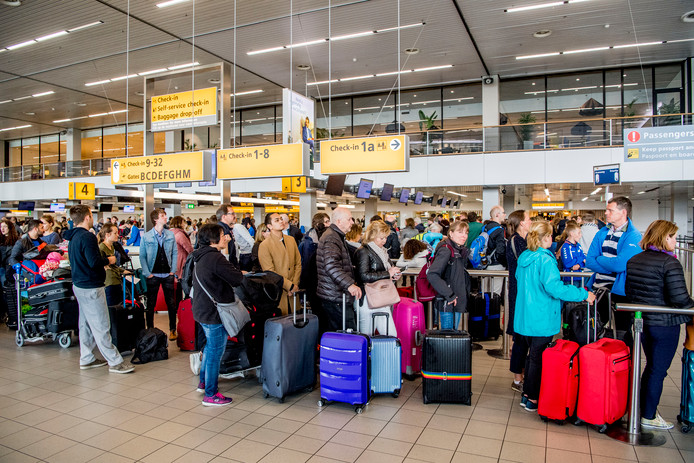
\includegraphics[width=\textwidth]{checkin}
Een rij mensen bij de incheckbalie van een luchthaven schuift meestal langzaam op richting knappe juffrouw met blauw pakje.
Ook alle koffers worden dan zuchtend weer een plaatsje naarvoren geschoven.
Bij gegevens in het hoofdgeheugen van een computer dient dit te worden voorkomen.
Alles vier bytes opschuiven bij een queue van twee gigabytes is een onnodig dure operatie.
Beter is 't de queue op z'n plek te laten en te onthouden waar de het eerste en 't laatste dataelement zich bevinden.
De dame van de incheckbalie loopt in dit geval langs de rij met een verrijdbare weegschaal voor de koffers en een labelprinter.
Wie is afgehandeld gaat uit de rij met z'n gewogen en gelabelde koffer en zet 'm ergens op een lopende band.
Op die plek waar mensen uit de rij gaan, komen er nieuwe mensen bij.
Niemand hoeft op te schuiven en iedereen kan rustig zittend op z'n koffer genieten van het uitzicht op alle rennende zakenlui.
Geen luchthaven is nog op dit idee gekomen, maar bij software queues is dit al lang gebruikelijk.}}

\paragraph{Oefening}

Maak een class \code{Queue} die de data niet opschuift, maar onthoudt waar er data bijkomt en waar deze aan de beurt is om uit de rij gehaald te worden.
Iets in de rij plaatsen gebeurt met \emph{put}, iets eruit halen gebeurt met \emph{get}.
Om deze opdracht te kunnen maken, kun je, naast een array, het beste de Java \emph{modulus} operator (\code{\%}) gebruiken.
Zoek op internet op hoe deze precies werkt.

Maak met behulp van je class \code{Queue} een class \code{Obfuscator}, een geheimtaalmachine die woorden op volgorde van aankomst omzet naar een onleesbare, maar decodeerbare string. Dit kan op allerlei manieren, bijvoorbeeld door iedere letter te vervangen door de letter die erna komt in het alfabet. Zo wordt ``java'' dan ``kbwb''.
Maak een hoofdprogramma dat een zin op deze manier codeert en de gecodeerde woorden afdrukt.
Het moet mogelijk zijn woorden in ``kluitjes'' in te voeren en ze er in andere ``kluitjes'' uit te halen.
Met andere woorden: je obfuscator moet op woordniveau kunnen bufferen:
net als bij printopdrachten komen de woorden in een queue te staan waar ze zo af en toe (eventueel in kluitjes) worden uitgehaald.

Bijvoorbeeld: je stopt eerst drie woorden in je \code{Obfuscator} met \emph{put} om gecodeerd te worden. Vervolgens haal je er twee gecodeerde woorden uit met \emph{get}. Dan stop je er weer één in en haal je er twee uit. 
Ook hier mag je weer dingen vragen en hulp zoeken.
Maar ook hier wordt weer van je verwacht dat je uiteindelijk regel voor regel kunt uitleggen hoe je code werkt.

\section{Class interaction}
Zorg dat de toestand (bewegingsrichting) van elk \code{motorizedWheel} gezet, onthouden en weer gelezen kan worden. De class moet daarvoor de methods \code{void forward()}, \code{void reverse()} en \code{void stop()} hebben, en de method \code{double getSpeed()}, die 10.0 teruggeeft als de motor in z'n vooruit staat, -10.0 als hij in z'n achteruit staat, en 0.0 als hij stilstaat. Bedenk of deze methods private of public moeten zijn en welke fields je nog meer nodig hebt, en of die private of public moeten zijn. Schrijf in class \code{Program} een stukje testcode voor beide wielen.

Zorg dat de positie en de ori"entatie van het voertuig onthouden en opgevraagd kunnen worden. De class \code{Vehicle} moet hiervoor een method \code{getPosition()} bevatten, die de huidige positie van het voertuig teruggeeft als een object van class \code{Position}. De class \code{Vehicle} moet ook een method \code{getOrientation()} bevatten, die de huidige ori"entatie van het voertuig teruggeeft in graden, als een \code{double} in de range 0--360.

Als het voertuig tegen een obstakel aanbotst, wordt de method \code{bounceBack(Position p)} aangeroepen. Deze moet dus ook aanwezig zijn in de class \code{Vehicle} en moet het voertuig terugplaatsen naar de aangegeven positie. Schrijf ook code om deze methods te testen.
\section{Updating}
Er moet in de class \code{Vehicle} een method \code{updateVehicle(double dt)} zijn die de positie en de ori"entatie aanpast op basis van de twee instanties van \code{MotorizedWheel}: \code{leftWheel} en \code{rightWheel}. Het argument \code{dt} is de duur van het tijdsstapje waarin gerekend wordt. Als beide motoren vooruit staan, beweegt het voertuig 10 pixels per seconde in de richting van de huidige ori"entatie. Als beide motoren achteruit staan, beweegt het voertuig 10 pixels per seconde in de richting tegengesteld aan de huidige oriëntatie. Als één van beide wielen beweegt en de ander staat stil, dan beweegt het voertuig 5 pixels per seconde (vooruit of achteruit, afhankelijk van de stand van de motor) en verandert de ori"entatie van het voertuig met 5\textdegree{} per seconde (linksom of rechtsom, afhankelijk van welke motor draait en welke kant op). Als beide motoren een tegengestelde richting op draaien, blijft de positie gelijk maar verandert de ori"entatie 10\textdegree{} per seconde. De positie en ori"entatie mogen alleen door deze method en door de method \code{bounceBack()} veranderd worden.

Rekenvoorbeeld: De huidige positie is (10.0, 10.0) en de huidige oriëntatie is 30\textdegree{}. \code{leftWheel} staat vooruit, \code{rightWheel} staat stil. De doorgegeven duur van de tijdstap \code{dt} is 0.1 s. Het voertuig gaat 5 • 0.1 = 0.5 eenheden vooruit. De nieuwe positie wordt dan (10.0 + 0.5 • cos(30\textdegree{}),10.0 + 0.5 • sin(30\textdegree{})) = (10.43,10.25). De nieuwe ori"entatie wordt 30\textdegree{} -- 5\textdegree{} • 0.1 = 29.5\textdegree{}.

Voor deze berekening kun je de volgende code gebruiken:
\begin{lstlisting}
position.x += Math.cos(Math.PI * orientation / 180.0) * dt * 
	(leftWheel.getSpeed() + rightWheel.getSpeed()) / 2;
position.y += Math.sin(Math.PI * orientation / 180.0) * dt * 
	(leftWheel.getSpeed() + rightWheel.getSpeed()) / 2;
orientation += 0.5 * dt * (rightWheel.getSpeed() - leftWheel.getSpeed());
orientation = (orientation + 360) % 360; // keep orientation within range 0-360
\end{lstlisting}
\section{Driving (inleveropgave, summatief)}
Maak een class \code{Program} met een static method \code{main()}. Deze method moet een instance van de classes \code{World} en \code{Vehicle} maken. Vervolgens moet de method \code{addVehicle(Vehicle v)} van de instance van \code{World} aangeroepen worden, met de instance van \code{Vehicle} als argument. Tenslotte moet de method \code{go()} van de instance van \code{World} aangeroepen worden.

De method \code{addSignal(Signal s)} van de class \code{Vehicle} wordt door de wereld herhaaldelijk aangeroepen met als argument een object van class \code{Signal} dat informatie bevat over de richting van en afstand tot obstakels in de omgeving en het doel. Voor ieder obstakel wordt er een apart \code{Signal} verstuurd. De richting is op te vragen met de method \code{double getAngle()}. Deze is ten opzichte van de huidige ori"entatie van het voertuig en loopt van -180\textdegree{} tot 180\textdegree{} (zie figuur). Een negatieve waarde betekent dat het obstakel zich rechts van de hartlijn van het voertuig bevindt. 0\textdegree{} is recht vooruit en een positieve waarde betekent dat het obstakel zich links van de hartlijn van het voertuig bevindt. De afstand is op te vragen met de method \code{double getDistance()}. Deze is ten opzichte van de huidige positie van het voertuig en houdt rekening met de afmetingen van voertuig en obstakel. E\'en van de signalen zal van het doel zijn waar het voertuig naartoe moet bewegen. De method \code{isTarget()} van een signaal levert \code{true} op als het het doel betreft, en anders \code{false}.\\
\centerline{\includegraphics[width=7cm]{signal}}

De class \code{Vehicle} moet een method \code{drive(double dt)} hebben. Deze wordt om de zoveel tijd aangeroepen met als argument de duur van de tijdstap \code{dt}. De bedoeling is dat deze method het voertuig bestuurt door de wielen (van class \code{MotorizedWheel}) aan te sturen (dat wil zeggen: vooruit, achteruit of stop te zetten) op basis van de binnengekomen signalen. Je kan er vanuit gaan dat tussen elke twee opeenvolgende aanroepen van \code{drive(double dt)} de signalen van alle obstakels in de wereld doorgegeven zijn. Bedenk zelf een slimme besturing en laat deze de methods \code{forward()}, \code{reverse()} en \code{stop()} van de wielen aanroepen. Vervolgens moet de method \code{updateVehicle(double dt)} aangeroepen worden (zie boven). De nieuwe positie en ori"entatie moeten elke keer naar een bestand weggeschreven worden (optioneel). De method \code{drive(double dt)} moet tenslotte de nieuwe positie van het voertuig teruggeven als een object van class \code{Position}.

Als het voertuig binnen 1 pixel van het doel gekomen is het doel bereikt en eindigt het programma. Hiervoor zorgt de class \code{World}.

Lever de code voor de classes \code{Program}, \code{Vehicle} en \code{MotorizedWheel} in, samen met een ontwerp, testplan en -rapport.
\newpage
\section*{Appendix: World.java}
\addcontentsline{toc}{section}{Appendix: World.java}
\lstinputlisting{World.java}
\end{document}